\documentclass{beamer}

\graphicspath{{img/}}

\usepackage{appendixnumberbeamer}

\usepackage{datetime}
\newdate{defensedate}{06}{09}{2017}
\newdate{startdate}{15}{05}{2017}
\newdate{enddate}{04}{08}{2017}

\usepackage{minted}

\usetheme[sectionpage=progressbar,subsectionpage=progressbar,numbering=fraction,
          progressbar=foot]{metropolis}

\title{Automated Test Data Generation for Dynamically-Typed Programming Languages}
\subtitle{Supervisor: Shin Yoo\\COINSE Lab, KAIST, South-Korea\\\displaydate{startdate} -- \displaydate{enddate}}

\date{\displaydate{defensedate}}
\author{%
  Simon Bihel\hfill\url{simon.bihel@ens-rennes.fr} \\
}
\institute{%
  University of Rennes I \\
  \'Ecole Normale Sup\'erieure de Rennes
}

\begin{document}

\maketitle

% \begin{frame}{Table of contents}
%   \setbeamertemplate{section in toc}[sections numbered]
%   \tableofcontents[hideallsubsections]
% \end{frame}


% \section*{Introduction}

\section{Automated Test Data Generation}

\begin{frame}{Tests are important}
  Tests are essentials. % to avoid bugs.
  % \begin{itemize}
  %   \item .
  % \end{itemize}

  But writing them by hand is:
  \begin{itemize}
    \item time-consuming,
    \item error-prone.
  \end{itemize}
\end{frame}

\begin{frame}{Test Data Generation}
  Generate inputs to satisfy some metrics for the System Under Test (e.g.\ a function, a class\dots).

  Examples of code coverage criteria:
  \begin{itemize}
    \item statement coverage,
    \item function coverage,
    \item branch coverage\dots
  \end{itemize}
\end{frame}

\begin{frame}[fragile]{Pathwise tests}
  \begin{columns}
    \begin{column}{0.5\textwidth}
      \begin{minted}{c}
int test(char x, char y) {
  if (x==y)
    printf("Equal");
  else
    printf("Not Equal");
  return 1;
}
      \end{minted}
    \end{column}
    \begin{column}{0.5\textwidth}
      Control flow graph

      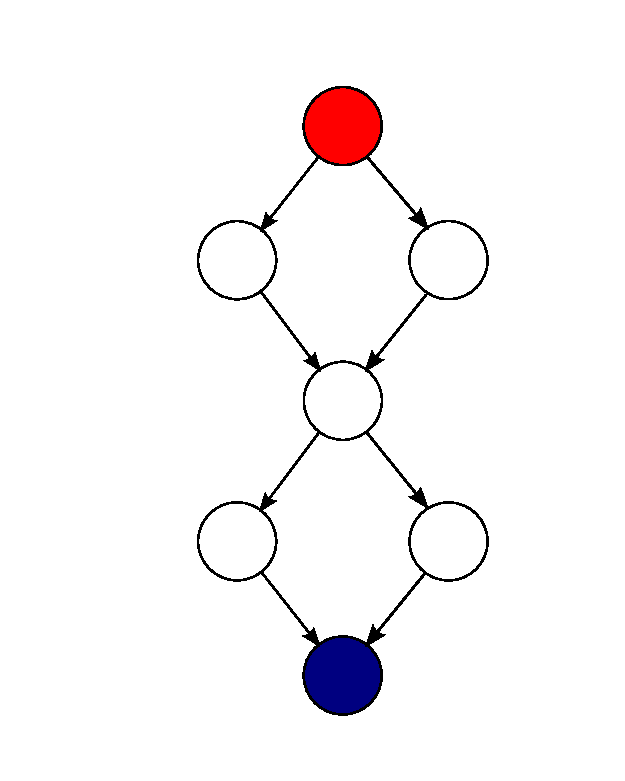
\includegraphics[height=0.6\textheight]{Control_flow_graph}
    \end{column}
  \end{columns}
\end{frame}

\begin{frame}{Search-Based Testing}
  \begin{enumerate}
    \item Inject code (instrument) in the SUT to measure metrics.
    \item Execute the SUT and get feedback.
    \item Modify inputs and re-execute the SUT.
  \end{enumerate}

  Search algorithms include: hill climbing, genetic algorithms\dots
\end{frame}


\section{A Tool for Dynamically-Typed Languages}

\begin{frame}{Background}
  \begin{itemize}
    \item Python tool
    \item Started as a fork of CAVM (a tool for \texttt{C})
  \end{itemize}

  Targets:
  \begin{itemize}
    \item find appropriate types;
    \item handle Python's lists (multi-types, unbounded).
  \end{itemize}
\end{frame}

\begin{frame}[fragile]{Big points of CAVM}
  \begin{columns}
    \begin{column}{0.5\textwidth}
      \begin{enumerate}
        \item Instrumentation of the source code to wrap conditions.
        \item Get distance to pass conditions.
        \item Use evolutionary techniques to tweak inputs.
      \end{enumerate}
    \end{column}
    \begin{column}{0.5\textwidth}
      \begin{minted}[escapeinside=||]{c}
int test(char x, char y) {
  if (|\colorbox{lime}{branchid(0, Eq(x, y))}|)
    printf("Equal");
  else
    printf("Not Equal");
  return 1;
}
      \end{minted}
    \end{column}
  \end{columns}
\end{frame}

\begin{frame}{Big points of the python tools}
  Additional instrumentation on element access to know which element is problematic in list.
\end{frame}

\begin{frame}{Identifiable Errors}

\end{frame}


\section{Challenges}

\begin{frame}{Dynamic types problems}
  \begin{itemize}
    \item Detect type errors bugs
    % \item Relations between parameters
    \item Working but unfit types (e.g.\ float instead of int)
    \item Difficulty to reduce domain of possible types
  \end{itemize}
\end{frame}

\begin{frame}{Bigger picture problems}
  Dynamic languages usually have other paradigms

  \begin{itemize}
    \item Controlling the environment
    \item Understanding results
    \item Infinite search spaces
    \item Dynamic data structures
    \item Dynamic insertion of code
    \item Objects state
  \end{itemize}
\end{frame}

\begin{frame}{Future work}
  \begin{itemize}
    \item Need of additional methods like a first round of static analysis.
  \end{itemize}
\end{frame}


\section*{Conclusion}

\begin{frame}{Conclusion}
  \begin{itemize}
    \item Search-based approach only seems unfeasible.
  \end{itemize}
\end{frame}


\end{document}
